\chapter{\TikZ}

\TikZ 是一個提供了繪畫功能的 package

\section{基礎使用}

有兩種方式使用 \TikZ 繪圖,第一是將命令放在 \verb`\tikz `後,第二是將命令用放在 tikzpicture 環境中

\begin{tcblisting}{listing only}
\tikz 命令
\begin{tikzpicture}
命令
\end{tikzpicture}
\end{tcblisting}

\subsection{直線}

在 \TikZ 中畫直線需要用到 \verb`\draw[選項]`這個命令

\begin{tcblisting}{listing only}
\draw[選項] ...... ;
\end{tcblisting}

如果想要畫一條直線,只需要在 \verb`\draw `的後面加上點的座標標,再由\-\- 連起來即可,最後不要忘記加上分號

\begin{tcblisting}{listing side text}
\tikz \draw (0,0)--(2,0)--(2,2);
\end{tcblisting}

我們可以將起點與終點的座標重疊,達成封閉圖形的效果

\begin{tcblisting}{listing side text}
\tikz \draw (0,0)--(2,0)--(2,2)--(0,0);
\end{tcblisting}

但這樣會有一個問題,如果你加入 [rounded corners] 這個讓原本鋒利的邊角變成圓角的參數時,你就會發現有問題

\begin{tcblisting}{listing side text}
\tikz \draw[rounded corners] (0,0)--(2,0)--(2,2)--(0,0);
\end{tcblisting}

這是因為圖片只有看起來是是封閉的,但 TikZ 並不認為他是一個封閉的圖形,這時候只需要在最後加入 \verb`--cycle` 就可以避免這個問題了

\begin{tcblisting}{listing side text}
\tikz \draw[rounded corners] (0,0)--(2,0)--(2,2)--cycle;
\end{tcblisting}

\subsection{矩形}

畫矩形也可以用上面的方式畫,但 \TikZ 有提供更簡單的方式

\begin{tcblisting}{listing side text}
\tikz \draw (0,0) rectangle (2,2);
\end{tcblisting}

你只需要在 rectangle 後放入對腳座標即可

\subsection{圓形、橢圓形、圓弧}

畫一個圓也非常簡單,先給出圓心再給出半徑,中間要加入 circle 將兩者隔開即可

\begin{tcblisting}{listing side text}
\tikz \draw (0,0) circle (2);
\end{tcblisting}

在上圖中的是一個圓心在 (0,0) 半徑為 2 的圓形,畫橢圓形與畫圓形類似,只不過需要把 circle 換成 ellipse ,且在指定長軸與短軸時需用 and 將兩者隔開

\begin{tcblisting}{listing side text}
\tikz \draw (0,0) ellipse (2 and 1);
\end{tcblisting}

圓弧則是將 circle 或 ellipse 換成 arc ,並需要額外指定角度

\begin{tcblisting}{listing side text}
\tikz \draw (0,0) arc (0:270:1);
\end{tcblisting}

上圖畫出了一個由 (0,0) 開始、從 0 度畫到 270 度、半徑為 1 的四分之三圓弧,橢圓形的圓弧當然也可以這樣畫出來

\begin{tcblisting}{listing side text}
\tikz \draw (0,0) arc (0:270:1 and 2);
\end{tcblisting}

\subsection{曲線}

曲線則是將直線中的 \verb`--` 換成 \verb`..` 就可以畫出貝茲曲線,也因為是畫出貝茲曲線,所以需要加入至少一個控制點

\begin{tcblisting}{listing side text}
\tikz \draw (0,0).. controls (1,1) ..(2,0);
\end{tcblisting}

多個控制點則需要用 and 區隔

\begin{tcblisting}{listing side text}
\tikz \draw (0,0).. controls (0.5,1) and (1.5,1) ..(2,0);
\end{tcblisting}

\subsection{格線}

格線則是利用 grid 來達成

\begin{tcblisting}{listing side text}
\tikz \draw (0,0) grid (2,2);
\end{tcblisting}

\subsection{極座標}

除了平面座標外也可以指定極座標

\begin{tcblisting}{listing side text}
\tikz \draw (0:0)--(45:1);
\end{tcblisting}

\section{可用的選項}

\TikZ\ 提供了大量的可自定義的選項,供使用者畫出自己想像中的圖片

\subsection{顏色}

顏色可以利用 draw 來決定

\begin{tcblisting}{listing side text}
\begin{tikzpicture}
\draw[draw = blue] (0,0)--(5,0);
\draw[draw = red] (0,-1)--(5,-1);
\draw[draw = yellow] (0,-2)--(5,-2);
\end{tikzpicture}
\end{tcblisting}

如果要填色,可以利用 fill 來填滿顏色,如果目前的圖形不是封閉圖形,那會自動變成封閉圖形

\subsection{粗細}

粗細可以利用 line width 來決定

\begin{tcblisting}{listing side text}
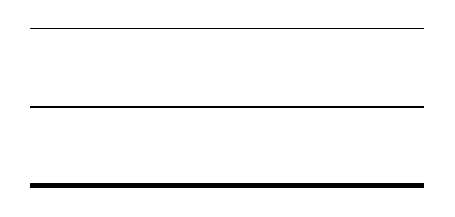
\begin{tikzpicture}
\draw (0,0)--(5,0);
\draw[line width = 1pt] (0,-1)--(5,-1);
\draw[line width = 2pt] (0,-2)--(5,-2);
\end{tikzpicture}
\end{tcblisting}

TikZ 的預設值是 0.4pt

\subsection{箭頭}

可以利用 > 與 < 來指定箭頭的形式

\begin{tcblisting}{listing side text}
\begin{tikzpicture}
\draw[-] (0,0)--(5,0);
\draw[<-] (0,-1)--(5,-1);
\draw[->] (0,-2)--(5,-2);
\draw[<->] (0,-3)--(5,-3);
\draw[|->] (0,-4)--(5,-4);
\draw[|<->|] (0,-5)--(5,-5);
\draw[|-|] (0,-6)--(5,-6);
\draw[->|] (0,-7)--(5,-7);
\draw[>->>] (0,-7)--(5,-7);
\end{tikzpicture}
\end{tcblisting}

上圖是一些示範

\subsection{預定義好的樣式}

TikZ 也有預先定義好一些樣式,讓我們可以使用

\begin{tcblisting}{listing side text}
\begin{tikzpicture}
\draw[dotted] (0,0)--(5,0);
\draw[densely dotted] (0,-1)--(5,-1);
\draw[loosely dotted] (0,-2)--(5,-2);
\draw[dashed] (0,-3)--(5,-3);
\draw[densely dashed] (0,-4)--(5,-4);
\draw[loosely dashed] (0,-5)--(5,-5);
\end{tikzpicture}
\end{tcblisting}

\subsection{平移、縮放與旋轉}

可以利用 shift 來達成平移的效果

\begin{tcblisting}{listing side text}
\begin{tikzpicture}
\draw (0,0) rectangle (1,1);
\draw[shift={(2,0)}] (0,0) rectangle (1,1);
\draw[shift={(2,2)}] (0,0) rectangle (1,1);
\draw[shift={(0,2)}] (0,0) rectangle (1,1);
\draw[shift={(-2,2)}] (0,0) rectangle (1,1);
\draw[shift={(-2,0)}] (0,0) rectangle (1,1);
\draw[shift={(-2,-2)}] (0,0) rectangle (1,1);
\draw[shift={(0,-2)}] (0,0) rectangle (1,1);
\draw[shift={(2,-2)}] (0,0) rectangle (1,1);
\end{tikzpicture}
\end{tcblisting}

\begin{itemize}
\item 第二個正方形的左下頂點由 (0,0) 移到了 (2,0)
\item 第三個正方形的左下頂點由 (0,0) 移到了 (2,2)
\item 第四個正方形的左下頂點由 (0,0) 移到了 (0,2)
\item 第五個正方形的左下頂點由 (0,0) 移到了 (-2,2)
\item 第六個正方形的左下頂點由 (0,0) 移到了 (-2,0)
\item 第七個正方形的左下頂點由 (0,0) 移到了 (-2,-2)
\item 第八個正方形的左下頂點由 (0,0) 移到了 (0,-2)
\item 第九個正方形的左下頂點由 (0,0) 移到了 (2,-2)
\end{itemize}

也可以在 shift 前加上 x 或 y 來決定平移的方向,但在這種情況下就不能使用內建的長度單位,需要自行指定

\begin{tcblisting}{}
\begin{tikzpicture}
\draw (0,0) rectangle (1,1);
\draw[xshift=100pt] (0,0) rectangle (1,1);
\draw[xshift=-100pt] (0,0) rectangle (1,1);
\draw[yshift=100pt] (0,0) rectangle (1,1);
\draw[yshift=-100pt] (0,0) rectangle (1,1);
\end{tikzpicture}
\end{tcblisting}

旋轉則需要利用 rotate

\begin{tcblisting}{}
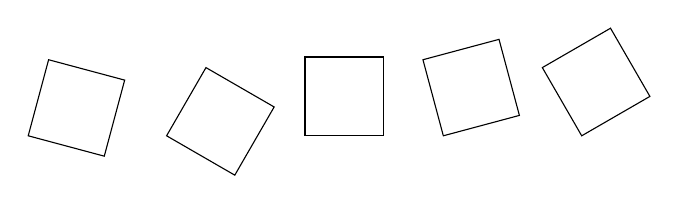
\begin{tikzpicture}
\draw (0,0) rectangle (1,1);
\draw[xshift=100pt, rotate=30] (0,0) rectangle (1,1);
\draw[xshift=50pt, rotate=15] (0,0) rectangle (1,1);
\draw[xshift=-100pt, rotate=-15] (0,0) rectangle (1,1);
\draw[xshift=-50pt, rotate=-30] (0,0) rectangle (1,1);
\end{tikzpicture}
\end{tcblisting}

\section{進階使用}

\subsection{節點}

在 \TikZ\ 中可以利用 \verb`\node(name) at(x,y) {text};` 放置節點

\begin{tcblisting}{listing side text}
\begin{tikzpicture}
\draw[help lines] (-2,-2) grid (2,2);
\node(1) at(0,0) {原點};
\end{tikzpicture}
\end{tcblisting}

想要連接兩個節點時,可以將座標改為兩個節點的名字

\begin{tcblisting}{listing side text}
\begin{tikzpicture}
\node(A) at(0,0) {A};
\node(B) at(2,0) {B};
\node(C) at(0,2) {C};
\draw (A)--(B)--(C);
\end{tikzpicture}
\end{tcblisting}

\verb`\node `如同 \verb`\draw `也可以使用選項來調整樣式

\begin{tcblisting}{listing side text}
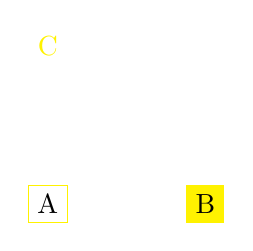
\begin{tikzpicture}
\node[draw=yellow](A) at(0,0) {A};
\node[fill=yellow](B) at(2,0) {B};
\node[text=yellow](C) at(0,2) {C};
\end{tikzpicture}
\end{tcblisting}

當然也有一些是只能用在 \verb`\node `上的選項

\begin{tcblisting}{listing side text}
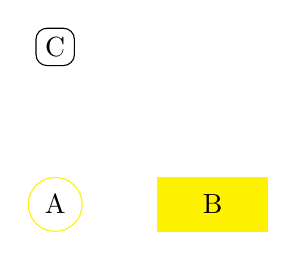
\begin{tikzpicture}
\node[draw=yellow,circle](A) at(0,0) {A};
\node[fill=yellow, minimum width=40pt, minimum height=20pt](B) at(2,0) {B};
\node[draw=black, rounded corners](C) at(0,2) {C};
\end{tikzpicture}
\end{tcblisting}

\begin{itemize}
\item 第一個節點用 circle 將外匡變成圓形的
\item 第二個節點用 minimum width/height 定義節點的最小長寬
\item 第三個節點用 rounded corners 把節點的邊角轉成圓角
\end{itemize}

但有時候我們並不想要直接把節點放到指定的座標,而是想放到該座標的上下左右,這個時候也可以利用 \TikZ\ 內建的選項來達成

\begin{tcblisting}{listing side text}

\begin{tikzpicture}
\node[left] at(0,0) {left};
\node[right] at(0,0) {right};
\node[above] at(0,0) {above};
\node[below] at(0,0) {below};
\draw[fill=black] (0,0) circle (.1);
\end{tikzpicture}
\end{tcblisting}

\begin{itemize}
\item 第一個節點在 (0,0) 的左邊
\item 第二個節點在 (0,0) 的右邊
\item 第三個節點在 (0,0) 的上方
\item 第四個節點在 (0,0) 的下方
\end{itemize}

\subsection{自定義樣式}

如果你圖片裡的節點畫線條都有相似的共同點,你可以在\verb`\begin{tikzpicture}` 後加一個方括號,並將共通的選項放在方括號中

\begin{tcblisting}{listing side text}
\begin{tikzpicture}[text = red]
\node[left, fill = yellow] at(0,0) {left};
\node[right, draw = black, line width =1pt] at(0,0) {right};
\node[above, text = blue] at(0,0) {above};
\node[below, draw = blue, circle] at(0,0) {below};
\end{tikzpicture}
\end{tcblisting}

如果你有一個很複雜的樣式,但又不是共通的,你可以利用 \verb`\tikzset{}` 來將複雜的樣式定義成一個選項

\begin{tcblisting}{listing only}
\tikzset{mynode/.style = {
draw = gray!70!black,
line width = 0.8pt,
fill = blue!30,
rounded corners,
inner sep = 6pt, %文字與邊匡的距離
minimum width = 40pt,
minimum height = 20pt}
}
\end{tcblisting}

使用時只要用 \verb`\node[mynode]` 即可

\tikzset{mynode/.style = {
draw = gray!70!black,
line width = 0.8pt,
fill = blue!30,
rounded corners,
inner sep = 6pt, %文字與邊匡的距離
minimum width = 40pt,
minimum height = 20pt}
}
\begin{tcblisting}{}
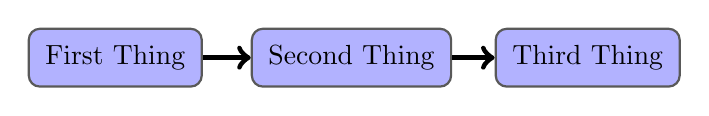
\begin{tikzpicture}[->, line width = 2pt]
\node[mynode] (1) at (0,0) {First Thing};
\node[mynode] (2) at (3,0) {Second Thing};
\node[mynode] (3) at (6,0) {Third Thing};
\draw (1)--(2);
\draw (2)--(3);
\end{tikzpicture}
\end{tcblisting}

這樣就方便許多了

\subsection{函數圖}

畫函數一樣是使用 \verb`\draw ` 這個命令

\begin{tcblisting}{}
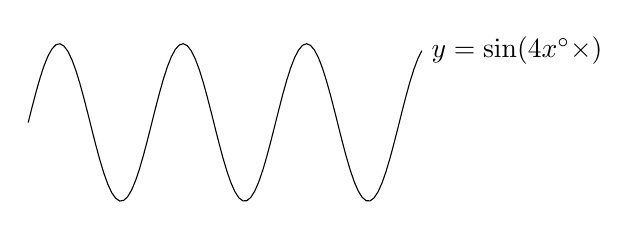
\begin{tikzpicture}
\draw[domain = 0:5, samples = 100] plot (\x,{sin(deg(\x*4))}) node[right] {$y=\sin(4x^\circ \times)$};
\end{tikzpicture}
\end{tcblisting}

domain 是我們要畫的區間,起點與終點要用冒號隔開,samples 決定圖形的精細程度,要特別注意的是需要運算的部分需要放在 \verb`{}`之間

\begin{figure}[htp]
\includegraphics[width=0.75\textwidth]{TikZ.png}
\end{figure}

上圖是可以使用的運算子,不過更複雜的函數圖形 \TikZ 就很難畫出來了,所以下一篇會介紹 pgfplots 這個 package
